\documentclass[12pt]{article}
\usepackage{amsmath}
\usepackage{fancyhdr}
\usepackage{amssymb}
\usepackage{amsthm}
\usepackage{graphicx}
\usepackage{varioref}
\usepackage{verbatim} 
\usepackage{multicol}
\usepackage{enumerate}
\usepackage[normalem]{ulem}
%\usepackage[margin=1in]{geometry}
\usepackage{caption}
\usepackage{subcaption}
\usepackage[T1]{fontenc}
\usepackage[margin=1in]{geometry}
\usepackage{thm-restate}
\usepackage{enumitem}
\usepackage{upgreek}
%\usepackage{cite}
\usepackage{cite}



\usepackage{mathrsfs}

\usepackage{url}\urlstyle{same}
\usepackage{xspace}
\usepackage{thm-restate}

% Nicer font
\usepackage{mathpazo}


% Microtype
\usepackage{microtype}

% TikZ
\usepackage{tikz}
\usetikzlibrary{calc}
\usetikzlibrary{decorations.pathmorphing}
\usetikzlibrary{decorations.markings}
\usetikzlibrary{graphs,graphs.standard,quotes}

% Support eps figures
\usepackage{epstopdf}

% Hypertext package
\usepackage[colorlinks = true]{hyperref}
% Title and authors
%\hypersetup{
%  pdftitle = {},
%  pdfauthor = {}
%}
% Color definitions
\usepackage{xcolor}
\definecolor{darkred}  {rgb}{0.5,0,0}
\definecolor{darkblue} {rgb}{0,0,0.5}
\definecolor{darkgreen}{rgb}{0,0.5,0}
% Color links
\hypersetup{
  urlcolor   = blue,         % color of external links
  linkcolor  = darkblue,     % color of internal links
  citecolor  = darkgreen,    % color of links to bibliography
  filecolor  = darkred       % color of file links
}

% Clever references
\usepackage{cleveref}%[nameinlink]
\crefname{lemma}{Lemma}{Lemmas}
\crefname{proposition}{Proposition}{Propositions}
\crefname{definition}{Definition}{Definitions}
\crefname{theorem}{Theorem}{Theorems}
\crefname{conjecture}{Conjecture}{Conjectures}
\crefname{corollary}{Corollary}{Corollaries}
\crefname{section}{Section}{Sections}
%\crefname{property}{Property}{Properties}
\crefname{appendix}{Appendix}{Appendices}
\crefname{figure}{Fig.}{Figs.}
\crefname{equation}{Eq.}{Eqs.}
\crefname{table}{Table}{Tables}
\crefname{claim}{Claim}{Claims}
%\crefname{item}{Property}{Properties}

%%%%%%%%%%%%%%%%%%%%%%%%%
%  N E W T H E O R E M  %
%%%%%%%%%%%%%%%%%%%%%%%%%

\newtheorem{theorem}{Theorem}
\newtheorem{lemma}[theorem]{Lemma}
\newtheorem{proposition}[theorem]{Proposition}
\newtheorem{definition}[theorem]{Definition}
\newtheorem{corollary}[theorem]{Corollary}
\newtheorem{conjecture}[theorem]{Conjecture}
\newtheorem{property}[theorem]{Property}
\newtheorem*{conjecture*}{Conjecture}
\newtheorem*{problem}{Problem}
\newtheorem{claim}[theorem]{Claim}
\theoremstyle{definition}
\newtheorem*{remark}{Remark}
\newtheorem*{example}{Example}

\DeclareMathOperator{\E}{\mathrm{E}}		     % expected value
\DeclareMathOperator{\Var}{\mathrm{Var}}         % variance
\DeclareMathOperator{\I}{\mathbb{1}}         % variance
\DeclareMathOperator{\pr}{\mathrm{P}}		     % expected value
\DeclareMathOperator{\cov}{\uptau_\textrm{cov}}  % cover time variable
\DeclareMathOperator{\tcov}{t_\textrm{cov}}      % cover time
\DeclareMathOperator{\hit}{t_{\textrm{hit}}}     % hitting time
\DeclareMathOperator{\tmina}{t_\textrm{min}^A}   % minimum time on A
\DeclareMathOperator{\Ceff}{C_\textrm{eff}}      % effective conductance
\DeclareMathOperator{\Reff}{R_{\textrm{eff}}}    % effective resistance
\DeclareMathOperator{\Rxy}{R_{\textrm{x,y}}}     % effective resistance between x,y
\DeclareMathOperator{\T}{\mathcal{T}}            % spanning tree


\newcommand{\todo}[1]{{\color{blue}{[{\bf todo:} #1]}}}

\begin{document}


%+Title
\title{Cover Times of Random Walks}


\author{R. Teal Witter}

\date{\today}
%\date{\today}



\maketitle
%-Title

\abstract{abstract}

\newpage
\tableofcontents

\newpage
\section{Introduction and Background}

"white screen" problem
numerous applications
many mathematical tools

\subsection{Motivation}
universal travel sequences
graph connectivity
protocol testing

\subsection{Definitions}
We consider an undirected, connected graph $G$ without self loops or multi-edges.
Let $V(G)$ be the set of vertices and let $E(G)$ be the set of edges on $G$.
Then $n$ is the number of vertices $|V(G)|$.
We say $i\sim j$ for $i$ and $j$ in the vertex set $V(G)$ if $(i,j)$ in $E(G)$.
Assume that each vertex is accessible from every other vertex.
That is, there is a set of edges from any $x$ to any $y$.
%Without loss of generality, we label the vertices $\{1, 2, 3, ..., n\}$.

Let $C_{i,j}$ be the non-negative weight of the edge between vertices $i$ and $j$.
We will mostly consider unweighted graphs
with $C_{i,j} = 1$ if $i \sim j$ and $C_{i,j} = 0$ otherwise.

Define the weight of vertex $i$ 
\begin{align}
C_i &= \sum_{j:i \sim j} C_{i,j}. \nonumber
\end{align}
In the unweighted case, $C_i$ is the degree of vertex $i$.

We consider a random walk $(X_t)$ on $G$.
Call $X_t$ the vertex that the walk is on at time $t$.
The random walker begins at vertex $X_0$.
At each step, the walker at vertex $i$ moves to neighboring vertex
$j$ with probability $c(i,j)/c(i)$.

Let $T_{j}$ be the number of steps until the first visit to $j$.
Formally,
\begin{align}
T_{j} &= \textrm{min} \left\{t > 0 : X_t = j \right\}. \nonumber
\end{align}
Let the hitting time $\hit$ be the maximum expected time between two vertices on $G$.
Note that $\E_i[T_j] = \E[T_j | X_0 = i]$.
Formally, 
\begin{align}
\hit &= \max_{i,j \in V(G)} \E_i[T_j]. \nonumber
\end{align}
Let the cover time variable $\cov$ be the first time all vertices have been
visited by the random walk $(X_t)$.
Formally, $\cov$ is the minimum time that for all $i \in V(G)$
there exists $t \leq \cov$ such that $X_t = i$.
We define the cover time as the expected value of $\cov$ from
the worst initial vertex.
Formally,
\begin{align}
\tcov &= \max_{j \in V(G)} \E_j[\cov] . \nonumber
\end{align}

\subsection{Electrical Networks \label{sec:electric}}

There are many connections between electrical networks
and random walks \cite{DS84}.
Physical properties like voltage, current, and resistance
all have probabilistic interpretations.
In this section, we explore electrical networks to build intuition about 
random walks.

So that the reader may more easily distinguish between
vertices, consider $x$ and $y$ in $V(G)$.
Recall that $C_{x,y}$ is the weight of the edge
between vertices $x$ and $y$, $C_x$ is the sum
of all $C_{x,y}$ where $x \sim y$, and the probability $\pr_{x,y}$
that we go from $x$ to $y$ is $C_{x,y}/C_x$.
For the rest of this section, we will call $C_{x,y}$
the conductance between $x$ and $y$.
Define the resistance $R_{x,y}$ between $x$ and $y$
as $1/ C_{x,y}$.

We now consider the distribution of the random
walk on the vertices of our graph.
Define the proportion $\pi_x$ of time we spend in $x$
as $C_x/C$ where $C=\sum_y C_y$.

We verify that $\pi$ is the stationary distribution
of $(X_t)$.
To begin,
\begin{align}
C_x \pr_{x,y} &= C_x \frac{C_{x,y}}{C_x} = C_{x,y} = C_{y,x} 
= C_y \frac{C_{y,x}}{C_y} = C_y \pr_{y,x}. \nonumber
\end{align}
Dividing by $C$ gives $\pi_x \pr_{x,y} = \pi_y \pr_{y,x}$.
(So $\pi$ satisfies detailed balance.)
Summing over $x$,
\begin{align}
\sum_x \pi_x \pr_{x,y} = \pi_y . \nonumber
\end{align}
Then $\pi \pr = \pi$ where $\pr$ is the matrix of transition probabilities.
It follows that $\pi$ is indeed the stationary distribution of $(X_t)$.

We now introduce voltage, current, and effective resistance.
Consider $a$ and $b$ in $V(G)$.
Set the voltage to be 1 at $a$ and 0 at $b$.
We may think of voltage as the probability we get to $a$ before $b$.
Probabilistically, of course $v_a = 1$ and $v_b=0$.
Voltage is a harmonic function so the voltage at every vertex $x$ in 
$V(G) \textbackslash \{a,b\}$ is determined by the boundary values
(at $a$ and $b$).

The current between two vertices is the product of the
difference in their voltages and the conductance of their edge.
We may think of current as the net number of movements through an edge.
Kirchoff's Current Law says that the sum of current on any vertex is 0.
Probabilistically, of course every time we enter a vertex we must also leave it.
Using Kirchoff's Current Law and the definition of current,
we justify the probabilistic interpretation of voltage
\begin{align}
\sum_y i_{x,y} &= 0 = \sum_y (v_x - v_y)C_{x,y} \nonumber \\
v_x \sum_y C_{x,y} &= \sum_y C_{x,y} v_y \nonumber \\
v_x &= \sum_y \frac{C_{x,y}}{C_x} v_y = \sum_y \pr_{x,y} v_y. \nonumber
\end{align}
We can probabilistically verify that $v_x = \sum_y \pr_{x,y} v_y$
using first step analysis on the probability of reaching $a$ before $b$.

\subsection{Outline}


\section{Cover Times of Structured Graphs}

\subsection{Small Example}
In general, it is always possible to find the exact cover time
of a graph using first step analysis.
We demonstrate the strategy on a small graph suggested by \cite{BH94}.

\cref{fig:example} shows our small graph and the first step analysis
for the random walk $(X_t)$ started from the top left vertex.
The black circle indicates the current vertex of the random walk
and the empty circles indicate the visited vertices.

For a graph with $n$ vertices, there are $n$ possible choices for the current
vertex and $2^{n-1}$ possible combinations of visited and unvisited vertices
for each one.
Of course, some cases are inaccessible by a random walk.
But even on \cref{fig:example} where we exploit symmetry,
there are almost a prohibitive number.
It is easy to see that the number of cases 
grows exponentially with the number of vertices.

\begin{figure}[ht]
	\centering
		\begin{tikzpicture} [
            > = stealth, % arrow head style
            shorten > = 1pt, % don't touch arrow head to node
            %auto,
            node distance = 3cm, % distance between nodes
            semithick % line style
        ]

			\tikzstyle{edge}=[draw,line width = .5pt,-,black!100]

			\node (m) at (-1.2,1.75) {
				\begin{tikzpicture}[scale = 3]
				    \tikzstyle{edge}=[draw,line width = .5pt,-,black!100]
				    \tikzstyle{current}=[draw,circle,fill=black,scale=.5]
				    \tikzstyle{visited}=[draw,circle,fill=white,scale=.5]
				    \draw[edge] (0,0) -- (0,1);
				    \draw[edge] (0,0) -- (1,0);
				    \draw[edge] (0,1) -- (1,0);
				    \draw[edge] (0,1) -- (1,1);
				    \draw[edge] (1,1) -- (1,0);
				    \node (l) at (.5, 1.1) {$\tcov$};
				    \node (bl) at (0,0) {};
				    \node[current] (tl) at (0,1) {};
				    \node (br) at (1,0) {};
				    \node (tr) at (1,1) {};;
				\end{tikzpicture}
			};
			\node (a) at (2,3) {
				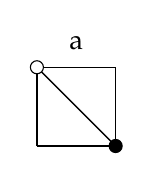
\begin{tikzpicture}[scale = 1]
				    \tikzstyle{edge}=[draw,line width = .5pt,-,black!100]
				    \tikzstyle{current}=[draw,circle,fill=black,scale=.5]
				    \tikzstyle{visited}=[draw,circle,fill=white,scale=.5]
				    \draw[edge] (0,0) -- (0,1);
				    \draw[edge] (0,0) -- (1,0);
				    \draw[edge] (0,1) -- (1,0);
				    \draw[edge] (0,1) -- (1,1);
				    \draw[edge] (1,1) -- (1,0);
				    \node (l) at (.5, 1.3) {a};
				    \node (bl) at (0,0) {};
				    \node[visited] (tl) at (0,1) {};
				    \node[current] (br) at (1,0) {};
				    \node (tr) at (1,1) {};;
				\end{tikzpicture}
			};
			\node (b) at (2,0) {
				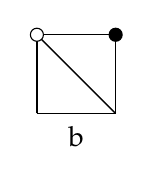
\begin{tikzpicture}[scale = 1]
				    \tikzstyle{edge}=[draw,line width = .5pt,-,black!100]
				    \tikzstyle{current}=[draw,circle,fill=black,scale=.5]
				    \tikzstyle{visited}=[draw,circle,fill=white,scale=.5]
				    \draw[edge] (0,0) -- (0,1);
				    \draw[edge] (0,0) -- (1,0);
				    \draw[edge] (0,1) -- (1,0);
				    \draw[edge] (0,1) -- (1,1);
				    \draw[edge] (1,1) -- (1,0);
				    \node (l) at (.5, -.3) {b};
				    \node (bl) at (0,0) {};
				    \node[visited] (tl) at (0,1) {};
				    \node (br) at (1,0) {};
				    \node[current] (tr) at (1,1) {};;
				\end{tikzpicture}
			};
			\node (c) at (4,3) {
				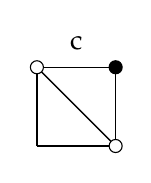
\begin{tikzpicture}[scale = 1]
				    \tikzstyle{edge}=[draw,line width = .5pt,-,black!100]
				    \tikzstyle{current}=[draw,circle,fill=black,scale=.5]
				    \tikzstyle{visited}=[draw,circle,fill=white,scale=.5]
				    \draw[edge] (0,0) -- (0,1);
				    \draw[edge] (0,0) -- (1,0);
				    \draw[edge] (0,1) -- (1,0);
				    \draw[edge] (0,1) -- (1,1);
				    \draw[edge] (1,1) -- (1,0);
				    \node (l) at (.5, 1.3) {c};
				    \node (bl) at (0,0) {};
				    \node[visited] (tl) at (0,1) {};
				    \node[visited] (br) at (1,0) {};
				    \node[current] (tr) at (1,1) {};;
				\end{tikzpicture}
			};
			\node (d) at (4,0) {
				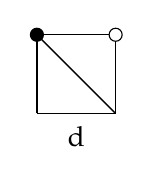
\begin{tikzpicture}[scale = 1]
				    \tikzstyle{edge}=[draw,line width = .5pt,-,black!100]
				    \tikzstyle{current}=[draw,circle,fill=black,scale=.5]
				    \tikzstyle{visited}=[draw,circle,fill=white,scale=.5]
				    \draw[edge] (0,0) -- (0,1);
				    \draw[edge] (0,0) -- (1,0);
				    \draw[edge] (0,1) -- (1,0);
				    \draw[edge] (0,1) -- (1,1);
				    \draw[edge] (1,1) -- (1,0);
				    \node (l) at (.5, -.3) {d};
				    \node (bl) at (0,0) {};
				    \node[current] (tl) at (0,1) {};
				    \node (br) at (1,0) {};
				    \node[visited] (tr) at (1,1) {};;
				\end{tikzpicture}
			};
			\node (e) at (6,3) {
				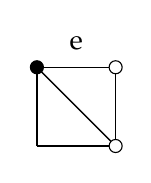
\begin{tikzpicture}[scale = 1]
				    \tikzstyle{edge}=[draw,line width = .5pt,-,black!100]
				    \tikzstyle{current}=[draw,circle,fill=black,scale=.5]
				    \tikzstyle{visited}=[draw,circle,fill=white,scale=.5]
				    \draw[edge] (0,0) -- (0,1);
				    \draw[edge] (0,0) -- (1,0);
				    \draw[edge] (0,1) -- (1,0);
				    \draw[edge] (0,1) -- (1,1);
				    \draw[edge] (1,1) -- (1,0);
				    \node (l) at (.5, 1.3) {e};
				    \node (bl) at (0,0) {};
				    \node[current] (tl) at (0,1) {};
				    \node[visited] (br) at (1,0) {};
				    \node[visited] (tr) at (1,1) {};;
				\end{tikzpicture}
			};		
			\node (f) at (6, 0) {
				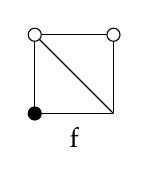
\begin{tikzpicture}[scale = 1]
				    \tikzstyle{edge}=[draw,line width = .5pt,-,black!100]
				    \tikzstyle{current}=[draw,circle,fill=black,scale=.5]
				    \tikzstyle{visited}=[draw,circle,fill=white,scale=.5]
				    \draw[edge] (0,0) -- (0,1);
				    \draw[edge] (0,0) -- (1,0);
				    \draw[edge] (0,1) -- (1,0);
				    \draw[edge] (0,1) -- (1,1);
				    \draw[edge] (1,1) -- (1,0);
				    \node (l) at (.5, -.3) {f};
				    \node[current] (bl) at (0,0) {};
				    \node[visited] (tl) at (0,1) {};
				    \node (br) at (1,0) {};
				    \node[visited] (tr) at (1,1) {};;
				\end{tikzpicture}
			};
			\node (done) at (8, 3) {
				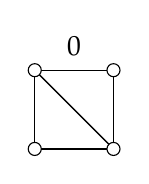
\begin{tikzpicture}[scale = 1]
				    \tikzstyle{edge}=[draw,line width = .5pt,-,black!100]
				    \tikzstyle{current}=[draw,circle,fill=black,scale=.5]
				    \tikzstyle{visited}=[draw,circle,fill=white,scale=.5]
				    \draw[edge] (0,0) -- (0,1);
				    \draw[edge] (0,0) -- (1,0);
				    \draw[edge] (0,1) -- (1,0);
				    \draw[edge] (0,1) -- (1,1);
				    \draw[edge] (1,1) -- (1,0);
				    \node (l) at (.5, 1.3) {0};
				    \node[visited] (bl) at (0,0) {};
				    \node[visited] (tl) at (0,1) {};
				    \node[visited] (br) at (1,0) {};
				    \node[visited] (tr) at (1,1) {};;
				\end{tikzpicture}
			};
			\node (g) at (8, 0) {
				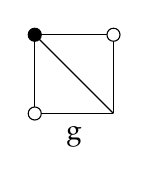
\begin{tikzpicture}[scale = 1]
				    \tikzstyle{edge}=[draw,line width = .5pt,-,black!100]
				    \tikzstyle{current}=[draw,circle,fill=black,scale=.5]
				    \tikzstyle{visited}=[draw,circle,fill=white,scale=.5]
				    \draw[edge] (0,0) -- (0,1);
				    \draw[edge] (0,0) -- (1,0);
				    \draw[edge] (0,1) -- (1,0);
				    \draw[edge] (0,1) -- (1,1);
				    \draw[edge] (1,1) -- (1,0);
				    \node (l) at (.5, -.3) {g};
				    \node[visited] (bl) at (0,0) {};
				    \node[current] (tl) at (0,1) {};
				    \node (br) at (1,0) {};
				    \node[visited] (tr) at (1,1) {};;
				\end{tikzpicture}
			};
			\begin{comment}
		    \path[->] (m) edge node[above] {$\frac{1}{3}$} (a);	
		    \path[->] (m) edge node[below] {$\frac{2}{3}$} (b); 
		    \path[->] (a) edge[loop above] node[below] {$\frac{1}{3}$} (a);
		    \path[->] (a) edge node[above] {$\frac{2}{3}$} (c);
		    \path[->] (b) edge[bend left] node[below] {$\frac{1}{2}$} (d);
		    \path[->] (b) edge node[below] {$\frac{1}{2}$} (e);
		    \path[->] (c) edge[bend left] node[above] {$1$} (e);
		    \path[->] (d) edge node[below] {$\frac{1}{3}$} (e);
		    \path[->] (d) edge[bend left] node[below] {$\frac{1}{3}$} (b); 
		    \path[->] (d) edge node[below] {$\frac{1}{3}$} (f);
		    \path[->] (e) edge[bend left] node[above] {$\frac{1}{3}$} (c);
		    \path[->] (e) edge[loop above] node[below] {$\frac{1}{3}$} (e);
		    \path[->] (f) edge[bend left] node[below] {$\frac{1}{2}$} (g);
		    \path[->] (g) edge[bend left] node[below] {$\frac{2}{3}$} (f);
			\path[->] (e) edge node[above] {$\frac{1}{3}$} (done);
			\path[->] (f) edge node[below] {$\frac{1}{2}$} (done);
			\path[->] (g) edge node[right] {$\frac{1}{3}$} (done);
			\end{comment}
			\path[->] (m) edge (a);
			\path[->] (m) edge (b);
			\path[->] (a) edge[loop above] (a);
			\path[->] (a) edge (c);
			\path[->] (b) edge[bend left] (d);
			\path[->] (b) edge (e);
			\path[->] (c) edge[bend left] (e);
			\path[->] (d) edge (e);
			\path[->] (d) edge[bend left] (b);
			\path[->] (d) edge (f);
			\path[->] (e) edge[bend left] (c);
			\path[->] (e) edge[loop above] (e);
			\path[->] (f) edge[bend left] (g);
			\path[->] (g) edge[bend left] (f);
			\path[->] (e) edge (done);
			\path[->] (f) edge (done);
			\path[->] (g) edge (done);
	\end{tikzpicture}
	\caption{First step analysis applied to a small graph with $n=4$.}\label{fig:example}
\end{figure}

If we let the label of each graph in \cref{fig:example}
denote the cover time from that case, we have the following system
of equations:
\begin{align}
\tcov &= 1 + \frac{1}{3}\textrm{a} + \frac{2}{3}\textrm{b} \nonumber \\
\textrm{a} &= 1 + \frac{1}{3}\textrm{a} + \frac{2}{3}\textrm{c} \nonumber \\
\textrm{b} &= 1 + \frac{1}{2}\textrm{b} + \frac{1}{2}\textrm{e} \nonumber \\
\textrm{c} &= 1 + 1\textrm{e} \nonumber\\
\textrm{d} &= 1 + \frac{1}{3}\textrm{a} + \frac{1}{3}\textrm{e} + \frac{1}{3}\textrm{f} \nonumber \\
\textrm{e} &= 1 + \frac{1}{3}\textrm{c} + \frac{1}{3}\textrm{e} + \frac{1}{3}\dot 0\nonumber \\
\textrm{f} &= 1 + \frac{1}{2}\textrm{g} + \frac{1}{2}\dot 0\nonumber \\
\textrm{g} &= 1 + \frac{2}{3}\textrm{f} + \frac{1}{3}\dot 0\nonumber
\end{align}

With a little linear algebra, we find that $\tcov = 43/6$.

For large graphs, the first step analysis as an approach to finding the expected
cover time is obviously intractable.
The rest of this section deals with particularly symmetric graphs
for which it is possible to find a solution for an arbitrary $n$.
However, we must rely on cover time bounds for the vast majority of cases.

\subsection{Complete Graph \label{sec:complete}}
We call the graph with an edge between each pair of vertices the
complete graph.
Note that a complete graph with $n$ vertices has ${n \choose 2}$ edges.

\begin{figure}[ht]
	\centering
	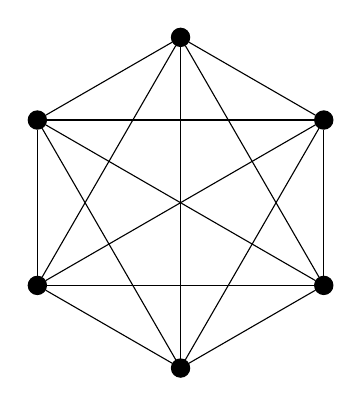
\begin{tikzpicture}[scale=.1]
	  \graph[circular placement, radius=3cm,
	         empty nodes, nodes={circle,draw,fill=black,scale=.7}] {
	    \foreach \x in {a,...,f} {
	      \foreach \y in {\x,...,f} {
	        \x -- \y;
	      };
	    };
	  };
	  \foreach \x [count=\idx from 0] in {a,...,f} {
	    \pgfmathparse{90 + \idx * (360 / 6)}
	    \node at (\pgfmathresult:4.4cm) {};
	  };
	\end{tikzpicture}
    \caption{The complete graph with six vertices (and ten edges).}\label{fig:complete}	
\end{figure}

Our goal is to find the expected number of steps until we have visited all
$n$ vertices in the complete graph.
Observe that the random walk can start at any vertex without loss of generality
because the graph is symmetric.
The strategy is to write the cover time $\tcov$ in terms of the expected
value of more simple random variables.
Let $X_i$ be the random variable that represents the number of steps to go
from $i-1$ to $i$ unique vertices (excluding the current vertex).

We write the cover time in terms of $X_i$ and use linearity of expectation.
\begin{align}
\tcov&= \E[X_1+X_2+X_3+...+X_{n+1}] = \sum_{i=1}^n \E[X_i] \nonumber
\end{align}

The random variable $X_i$ takes value $k$ when $k-1$ steps lead us to
already visited vertices and the $k^{th}$ step is to a previously unvisited vertex.
Then $X_i$ is certainly geometric and $\E[X_i] = 1/p_i$. 

\begin{comment}
It follows that $X_i$ is geometric with distribution
\begin{align}
\pr(X_i = k) = (1-p_i)^{k-1}p_i, \nonumber
\end{align}
where $p_i$ is the probability of moving to a previously unvisited vertex.
\end{comment}
We now find the probability $p_i$ that 
we go to a previously unvisited vertex is $(n-i)/(n-1)$.
This is because there are $n-i$ unvisited vertices and a total of $n-1$ adjacent vertices.
It follows that $\E[X_i] = (ln-1)(n-i)$.
Then
\begin{align}
\tcov&=   \sum_{i=1}^n \frac{n-1}{n-i} \nonumber \\
&=  (n-1) \left(\frac{1}{n-1}+\frac{1}{n-2}+...+1\right). \nonumber
\end{align}

A natural interpretation of the cover time on a complete graph is 
the so-called coupon collecting problem.
There are $r$ different coupons that are randomly packaged in cereal boxes.
An avid fan buys a box of cereal every day.
We want to know how many days until the fan has collected each coupon.
The strategy is to think of every coupon as a vertex on the complete graph.
We then move from vertex to vertex with uniform probability.
The difference between the coupon collecting problem and the complete graph
is that we now have self-edges.
Before, we had to leave our current vertex at each step.
Now, we can stay in the same vertex (provided our collector found the same coupon
two days in a row).
We apply our approach to the complete graph and substitute the $r$ possible coupons
we can find for the $n-1$ vertices we could move to.
Then
\begin{align}
\tcov&=  r \left(\frac{1}{r}+\frac{1}{r-1}+...+1\right). \nonumber
\end{align}

Another more subtle application of the cover time on a complete graph
is the cover time on an $n$-star.

\begin{figure}[ht]
	\centering
	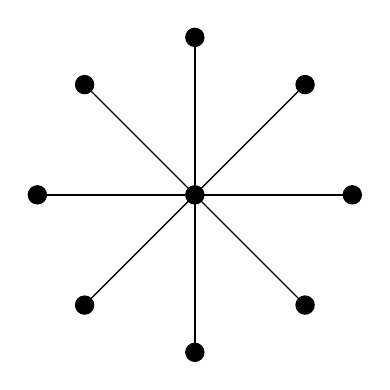
\begin{tikzpicture}[scale = 2]
	    \tikzstyle{vertex}=[draw, circle,fill=black, scale=.7]
	    \tikzstyle{edge}=[draw,line width = .5pt,-,black!100]
	    \node[vertex] (0) at (0,0) {};
	    \node[vertex] (1) at (1,0) {};
	    \node[vertex] (2) at (.7,-.7) {};
	    \node[vertex] (3) at (0,-1) {};
	    \node[vertex] (4) at (-.7,-.7) {};
	    \node[vertex] (5) at (-1,0) {};
	    \node[vertex] (6) at (-.7,.7) {};
	    \node[vertex] (7) at (0,1) {};
	    \node[vertex] (8) at (.7,.7) {};
	    \draw[edge] (1) -- (0);
	    \draw[edge] (2) -- (0);
	    \draw[edge] (3) -- (0);
	    \draw[edge] (4) -- (0);
	    \draw[edge] (5) -- (0);
	    \draw[edge] (6) -- (0);
	    \draw[edge] (7) -- (0);
	    \draw[edge] (8) -- (0);
	\end{tikzpicture}
	\caption{The nine-star.}\label{fig:n-star}
\end{figure}

An $n$-star is a graph with one central vertex and $n-1$ adjacent vertices each with a single
edge to the center.
A random walk begins at the central vertex and moves with uniform probability to
one of the $n-1$ adjacent vertices.
Whereas in the complete graph and coupon collecting problems we 
visited a (possibly) new vertex in one step,
a random walk on the $n$-star visits a (possibly) new vertex
in two steps: one step to each leaf and one step back.
We apply our approach to the complete graph and conclude that

\begin{align}
\tcov&= 2(n-1) \left(\frac{1}{n-1}+\frac{1}{n-2}+...+1\right). \nonumber
\end{align}

\subsection{Line Graph}
A line graph is a set of vertices connected in a line.
(\cref{fig:line} is an example with $n=N+1$.)

Our goal is to determine the cover time of a line graph.
Let $(X_t)$ be the random walk started at vertex $i$.
Notice that a random walk will have covered all vertices
exactly when it has visited both endpoints.
We can use this observation to break up the cover time into the time it takes
to reach one of the endpoints and the time it takes to reach 
the other endpoint.

We will begin by considering the time $(X_t)$ takes to
visit either one of the endpoints from vertex $i$.

From $X_t=i$, we move with equal probability to $i+1$
and $i-1$ until we reach either $0$ or $N$.

\begin{figure}[ht]
	\centering
	\begin{tikzpicture}
  		\pgfmathsetmacro{\N}{5}
		\tikzstyle{vertex}=[draw, circle,fill=black, scale=.7]
	    \tikzstyle{edge}=[draw,line width = .5pt,-,black!100]
		\tikzstyle{label}=[scale=.7]
		\draw[edge] (-\N,0) -- (\N,0);

		\node[label] (0) at (-\N,.5) {$0$};	
		\node[label] (N) at (\N,.5) {$N$};	
		\node[label] (0) at (-\N/5,.5) {$i$};

		\draw (-\N/5,0.1) -- (-\N/5,-0.1);
		\draw (\N,0.1) -- (\N,-0.1);
		\draw (-\N,0.1) -- (-\N,-0.1);

		\draw[edge] (-\N,0) -- (\N,0);
	\end{tikzpicture}
	\caption{A   line graph with a vertex at each integer from $0$ to $N$.}\label{fig:line}
\end{figure}

Call $e_i$ the expected number of steps until we reach either
end of our random walk from state $i$.
Our strategy is to write and solve a recurrence relation that
uses what we know about the random walk.
If $i=0,N$, we are already at the endpoint and $e_i=0$.
Otherwise, we take a step.
There's a half probability our step is to the right and
a half probability it is to the left.

\begin{align}
e_i &= 1 + \frac{1}{2} \left(e_{i+1}\right) + \frac{1}{2}\left(e_{i-1}\right) \nonumber \\
2 e_i &= 2 + e_{i+1} - e_{i-1} \nonumber \\
\left(e_{i+1} - e_i\right) &=\left( e_i - e_{i-1}\right) - 2 \nonumber
\end{align}

While the final line may look more complicated than what we started with,
notice that the structure of the equality lends itself to telescoping.

To solve the telescoping equations, observe that the walk is symmetric:
we could flip the walk over the vertical axis without changing $e_i$.
This makes sense because our intuition tells us that the only 
identifying feature of $i$ is its respective distances to the endpoints.
The logical conclusion is that $e_i=e_{N-i}$.
In particular, we have already seen that $e_0=e_N=0$ and it
naturally follows that $e_1=e_{N_1}$.
We use these observations to find $e_1$:

\begin{align}
(e_2 - e_1) &= (e_1-e_0) -2 \nonumber\\
(e_3 - e_2) &= (e_1-e_0) -4 \nonumber\\
&\;\;\vdots \nonumber\\
\left(e_N - e_{N-1}\right) &= \left(e_1 - e_0\right) - 2 (N-1) \nonumber \\
\left(0 - e_1\right) &= \left(e_1 - 0\right) - 2 (N-1) \nonumber \\
e_1 &= N-1. \nonumber
\end{align}

(Note that the vertical dots denote inductive reasoning.)
We now know $e_1$.
However, our goal is to find the expected number of steps
from an arbitrary point $i$.
We use $e_1$ to find the general solution.

\begin{comment}
\begin{align}
e_2  &= e_1 + (e_1 - e_0) - 2 = 2 (N - 2) \nonumber\\
e_3  &= e_2 + (e_2 - e_1) - 2 = 2 \left[2 (N-2) \right] - (N-1) -2 = 3 (N - 3) \nonumber\\
&\;\;\vdots \nonumber\\
e_i &= i (N-i) \label{eq:line}
\end{align}
\end{comment}

\begin{align}
(e_2 - e_1) &= (e_1-e_0) -2 \nonumber\\
(e_3 - e_2) &= (e_1-e_0) -4 \nonumber\\
&\;\;\vdots \nonumber\\
(e_i-e_{i-1}) &= (e_1 - e_0) - 2(i-1) \nonumber
\end{align}

Remember that $e_0=0$, $e_1=N-1$, and 
$\sum_{i}^{i-1} i = (i-1)i/2$.
We add all $i-1$ equations:

\begin{align}
(e_i - e_1) &= (i-1) e_1 - 2[1+2+...+i-1] \nonumber \\
e_i &= i(N-1) - 2 \frac{(i-1)i}{2} \nonumber\\
&= i(N-1 - i + 1) = i(N-i)
\label{eq:line}
\end{align}



\cref{thm:line} follows from \cref{eq:line} and the observation that any
line graph can be shifted so that the left endpoint
is at $0$ and the right endpoint is at $N$.

\begin{theorem}
The expected number of steps from a state to either end of a line graph
is the product of the distances from that state to each endpoint.
\label{thm:line}
\end{theorem}

We have the expected time until we reach one endpoint of our line graph.
Now we want to find the expected time from one endpoint to the other $\E_0[T_N]$.
By symmetry, $\E_0[T_N] = \E_N[T_0]$.

We write
\begin{align}
\E_0[T_N] &= \E_0[T_1] + \E_1[T_2] + ... + \E_{i}[T_{i+1}] + ... + \E_{N-1}[T_N]. \nonumber
\end{align}

where $\E_{i}[T_{i+1}]$ is the expected time from state $i$ to $i+1$.
Since there is only one edge incident to 0, we always move from 0 to 1.
From state $i\neq0$, we take one step in each direction with equal probability.
In half the cases, we have arrived at $i+1$.
In the other half of cases, we are in $i-1$.
It will take us $\E_{i-1}[T_i]$ steps back to $i$ and then another
$\E_i[T_{i+1}]$ steps to $i+1$.
Formally,
\begin{align}
\E_{i}[T_{i+1}] &= 1 + \frac{1}{2}(\E_{i-1}[T_i]+\E_i[T_{i+1}]) \nonumber \\
 &= 2 + \E_{i-1}[T_{i}]. \nonumber
\end{align}

We can use $\E_0[T_1] = 1$ to solve for $E_i[T_{i+1}]$:
\begin{align}
E_i[T_{i+1}] &= E_{i-1}[T_{i}] + 2 = E_{i-2}[T_{i-1}] + 4 \nonumber\\
 &= E_0[T_1] + 2(i-1) = 2i - 1. \nonumber
\end{align}

Then
\begin{align}
\E_0[T_N] &= 1 + 3 + ... + 2i - 1 + ... + 2(N-1) -1 \nonumber \\
&= N^2 \nonumber
\end{align}

Then, by \cref{thm:line}, for the random walk from state $i$ on the line graph,
\begin{align}
\tcov = i(N-i) + N^2. \nonumber
\end{align}

\subsection{Simple Cycle}

A simple cycle is a connected graph where
each vertex has an edge to exactly two other vertices.
(\cref{fig:cycle} is an example.)

Consider a random walk on a simple cycle as in \cref{fig:cycle}.
(Note that the starting vertex is arbitrary since the graph is symmetric.)
Let $(X_t)$ be the walk on the number line (between $-n$ and $n$)
where $X_0 = 0$.
The cover time $\tcov$ of the simple cycle is the expected number of steps 
until we visit $n$ distinct integers.

\begin{figure}[ht]
	\centering
	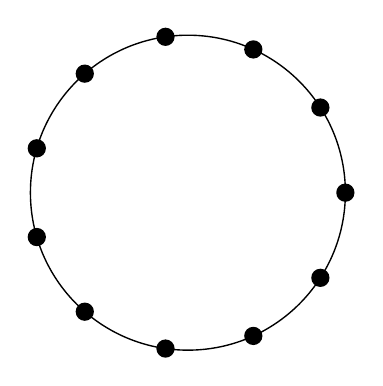
\begin{tikzpicture}
	\draw[line width=.5pt] circle (2cm);
	\foreach \a in {1,2,...,11} {
		\draw (\a*360/11: 2cm) node [circle, fill=black, scale=.7] (\a) {};
	}
	\end{tikzpicture}
	\caption{A cycle graph with $n=11$ vertices.}\label{fig:cycle}
\end{figure}

Let $\{a, a+1, \dots, b-1, b\}$ 
denote the set of vertices we have visited.
Since the walk is on a line, we can $[a,b]$ for the range
of the walk where $a$ is the smallest 
and $b$ is the largest vertex we have visited.
Notice that if $a \leq -n$ or $b \geq n$, we have covered all $n$ vertices
on the simple cycle and conclude the random walk.

In a slight abuse of notation, let $T_k$ be the 
number of steps until we reach $k$ distinct vertices.
Formally, $T_k = \min\{t: b-a+1 = k\}$.
Then by telescoping,
\begin{align}
\tcov &= \E[T_n] = \E[(T_2 - T_1) + (T_3 - T_2) + \dots + 
(T_k - T_{k-1}) + \dots + (T_n - T_{n-1})] \nonumber
\end{align}

At time $T_{k}$, we are either at integer $a$ or $b$.
Then $\E[T_{k+1}-T_{k}]$ is the first time we reach $a-1$ or $b+1$.
Notice that we can shift our endpoints to 0 and $b+1-(a-1) = b-a + 2 = k+1$.
The expected number of steps to either $a-1$ or $b+1$
is $1\dot (k+1-1) = k$ by \cref{thm:line}.

By linearity of expectation,
\begin{align}
\tcov &=  (\E[T_2] - \E[T_1]) + \dots +
(\E[T_{k+1}] - \E[T_{k}]) + \dots + (\E[T_n] - \E[T_{n-1}]) \nonumber\\
&= 1 + 2 + \dots + k-1 + \dots + n-1  = \frac{1}{2}n(n-1). \nonumber
\end{align}

\section{Bounds}

\subsection{Commute Time Identity} \label{sec:commute}
We use the electrical network analysis in \cref{sec:electric} to 
prove the commute time identity so we may use it to help us bound
cover times.

Define the probability $\pr_a(T_b < T_a)$ that starting at $a$
we reach $b$ before returning to $a$.
(Recall that $T_a>0$.)
Now define the effective conductance $\Ceff$ as $i_a/v_a$
and the effective resistance $\Reff$ as $1/\Ceff$.

With a voltage of 1 at $a$ and 0 at $b$,
\begin{align}
\Ceff &= i_a/1 =
\sum_y (v_a - v_y) C_{a,y} =
\sum_y (v_a - v_y) \frac{C_{a,y}}{C_a} C_a \nonumber \\
&= C_a (\frac{v_a}{C_a} \sum_y C_{a,y} - \sum_y \frac{C_{a,y}}{C_a} v_y)=
C_a(1-\sum_y\pr_{a,y}v_y).\nonumber
\end{align}

Recall $\sum_y P_{a,y} v_y$ is the probability we reach $a$ before $b$
so 1 minus that is the probability we reach $b$ before returning to $a$.

Then
\begin{align}
\Ceff = C_a \pr_a(T_b < T_a) \nonumber
\end{align}
and
\begin{align}
\Reff = \frac{1}{C_a \pr_a(T_b < T_a)}. \nonumber
\end{align}

We use the fact that $\pi_a = C_a / C$ and multiply by $C$,
\begin{align}
\Reff C = \frac{1}{\pi_a \pr_a(T_b < T_a)}. \nonumber
\end{align}

Recall that $\pr_a(T_b < T_a)$ is the probability, starting from $a$,
that we get to $b$ before returning to $a$.
We do independent trials, starting from $a$, until we reach $b$ before $a$.
Each ``failure'' resets the process so $\pr_a(T_b < T_a)$ is geometrically distributed.
Then the expected value $1/\pr_a(T_b < T_a)$ is the expected number of times
we return to $a$ before we finally reach $b$ (and again return to $a$).

Recall that $\pi_a$ is the probability that $(X_t) = a$.
By a similar argument, $1/\pi_a$ is the expected return time to $a$.

Thus the expected time from $a$ to $b$ and back is
the expected number of returns to $a$ before we reach $b$ times
the expected number of steps for each return to $a$.
The commute time identity follows
\begin{align}
E_a[T_b] + E_b[T_a] = \frac{1}{\pi_a}\frac{1}{\pr_a(T_b < T_a)} = \Reff C.
\label{eqn:commute}
\end{align}

\subsection{Matthews Method}
We have seen that it is in general very hard
to calculate the cover time of a random walk
on a graph.
The exceptions are symmetric or small graphs.
In lieu of an exact solution, we want to 
bound the cover time.

The Matthews Method is an example of a remarkably good bound \cite{LP17}.
In fact, it is tight for the complete graph:
the expected time between any two vertices
is $n-1 = \hit$ and \cref{thm:matthews_up} gives
us the main result of \cref{sec:complete}.

An added benefit is that the proof uses strategies we employed on the
simple cycle and follows an intuitive structure.

\begin{theorem}[Matthews Upper Bound]
Let $(X_t)$ be a random walk on a graph with $n$ vertices. Then \label{thm:matthews_up}
\end{theorem}
\begin{align}
\tcov &\leq \hit \left(1 + \frac{1}{2} + \frac{1}{3} + ... + \frac{1}{n-1} \right). \nonumber
\end{align}

\begin{proof}
Without loss of generality, label the vertices $\{1, 2, ..., n\}$.
We may assume that the walk started at vertex $n$.
Let $\sigma$ be a uniform permutation of the unvisited $n-1$ vertices.
The strategy is to look for the vertices in order $\sigma$.

Let $T_k$ be the first time that vertices $\sigma_1, \sigma_2, ..., \sigma_k$
have all been visited.
For ease of notation, set $L_k = X_{T_k}$ to be the last state among 
$\sigma_1, \sigma_2, ..., \sigma_k$ to be visited the first
time they are all visited.

We begin by writing the cover time in a clever way
(similar to the strategy we employed on the cycle graph):
\begin{align}
\tcov &= \E_n[{T_{n-1}}]  \nonumber \\
&= \E_n[T_1 + (T_2 - T_1) + ... + 
(T_k - T_{k-1}) + ... + (T_{n-1} - T_{n-2})] . \nonumber
\end{align}

Our goal is to bound the cover time in terms of the hitting time.

Consider the first term of the sum.
Recall that the hitting time $\hit$ is the maximum
expected time from any vertex to any other.
It follows that for any choice of $\sigma_1$,
the expected time from $n$ to $\sigma_1$ is less than or equal to $\hit$.
Formally for $s$ an arbitrary state such that $1\leq s \leq n-1$,
$\E_n[T_1] = \E_n[T_s] \leq \hit$.

Now consider the $k^{th}$ term of the sum for $1 < k \leq n-1$.
By conditional expectation,

\begin{align}
\E_n[T_k - T_{k-1}] &=
\sum_{i=1}^k \E_n[T_k - T_{k-1} | L(k) = \sigma_i]
P(L_k = \sigma_i). \nonumber 
\end{align}

Assume that the last vertex $L_k$ to be visted among the first
$k$ vertices is not $\sigma_k$.
Then the first time we visit the first $k-1$ vertices
is also the first time we visit the first $k$ vertices
(since we must have already visited $\sigma_k$).
Formally, $\E_n[T_k-T_{k-1}|L(k) \neq \sigma_k] = 0$.
Then 

\begin{align}
\E_n[T_k - T_{k-1}] &= 0 +
\E_n[T_k - T_{k-1} | L(k) = \sigma_k]
P(L_k = \sigma_k). \nonumber 
\end{align}

Since $\sigma$ is a random permutation, the probability that
we visit $\sigma_k$ last is $1/k$.
Formally, $P(L_k = \sigma_k) = 1/k$.

Finally, we find the expected time between $T_{k-1}$ and $T_{k}$
given that last vertex we visit is $\sigma_k$.
Consider $r$ and $s$ where $1 \leq r \neq s \leq n-1$
such that $L_{k-1} = r$ and $L_k = s$.
Then $\E_n[T_k - T_{k-1} | L(k) = \sigma_k] = \E_r[T_s] \leq \hit$.
So
\begin{align}
\E_n[T_k - T_{k-1}] &\leq
\hit \frac{1}{k}. \nonumber 
\end{align}

Putting it all together,
\begin{align}
\tcov \leq \hit \left( 1+ \frac{1}{2} + ... + \frac{1}{k} 
+ ... + \frac{1}{n-1} \right). \nonumber
\end{align}
\end{proof}

The same strategy for the Matthews upper bound can be used
to find a lower bound.
Instead of looking for all $n$ vertices, we search
for $A \subseteq V(G)$.
When the hitting time is large between any two vertices in $A$,
the time to visit all of $A$ is a good lower bound on the cover time
of $V(G)$.

\begin{theorem}[Matthews Lower Bound]
Let $A \subseteq V(G)$. Define $\tmina = \min_{a,b\in A, a \neq b} \E_b[T_a]$.
Let $(X_t)$ be a random walk on a graph with $n$ vertices. Then \label{thm:matthews_low}
\end{theorem}
\begin{align}
\tcov &\geq \tmina \left(1 + \frac{1}{2} + \frac{1}{3} + ... +
\frac{1}{|A| -1} \right). \nonumber
\end{align}

\begin{proof}
Without loss of generality, label the vertices $\{1, 2, ..., n\}$.
We may assume that the walk started at vertex $x \in A$.
Let $\sigma$ be a uniform permutation of the vertices in $A$.
The strategy is to look for the vertices in order $\sigma$.

Let $T_k$ be the first time that vertices $\sigma_1, \sigma_2, ..., \sigma_k$
have all been visited.
For ease of notation, set $L_k = X_{T_k}$.

We again write the cover time in a clever way:
\begin{align}
\tcov &\geq \E_x[T_1 + (T_2 - T_1) + ... + 
(T_k - T_{k-1}) + ... + (T_{|A|} - T_{|A|-1})] . \nonumber
\end{align}

Our goal is to bound the cover time in terms of $\tmina$.

Consider the first term of the sum.
With probability $1/|A|$, $\sigma_1 = x$ and $T_1=0$.
Otherwise, the expected time from $x$ to $T_1$ is less than or equal to
$\tmina$.
Then
\begin{align}
\E_x[T_1] \geq \frac{1}{|A|}0 + \frac{|A| -1}{|A|} \tmina
= \left(1 - \frac{1}{|A|} \right) \tmina \nonumber
\end{align}

Now consider the $k^{th}$ term of the sum for $k > 1$.
By conditional expectation,
\begin{align}
\E_x[T_k - T_{k-1}] &=
\sum_{i=1}^k \E_x[T_k - T_{k-1} | L(k) = \sigma_i]
P(L_k = \sigma_i). \nonumber 
\end{align}

Assume that the last vertex $L_k$ to be visted among the first
$k$ vertices is not $\sigma_k$.
Then $\E_x[T_k-T_{k-1}|L(k) \neq \sigma_k] = 0$.
It follows that
\begin{align}
\E_x[T_k - T_{k-1}] &= 0 +
\E_x[T_k - T_{k-1} | L(k) = \sigma_k]
P(L_k = \sigma_k). \nonumber 
\end{align}

Since $\sigma$ is a random permutation, $P(L_k = \sigma_k) = 1/k$.

Now find the expected time between $T_{k-1}$ and $T_{k}$
given that last vertex we visit is $\sigma_k$.
Consider $r, s \in A$ such that $L_{k-1} = r$ and $L_k = s$.
Then $\E_x[T_k - T_{k-1} | L(k) = \sigma_k] = \E_r[T_s] \geq \tmina$.
So
\begin{align}
\E_x[T_k - T_{k-1}] &\geq
\tmina \frac{1}{k}. \nonumber 
\end{align}

Putting it all together,
\begin{align}
\tcov &\geq \tmina \left( 1 - \frac{1}{|A|}+ \frac{1}{2} + ... + \frac{1}{k} 
+ ... + \frac{1}{|A|-1} + \frac{1}{|A|}\right). \nonumber \\
&= \tmina \left( 1 + \frac{1}{2} + ... + \frac{1}{k} 
+ ... + \frac{1}{|A|-1} \right). \nonumber
\end{align}
\end{proof}

\subsection{Matthews Method on Binary Trees}
\todo{graph example of binary tree}

\cite{LP17}
Consider a complete unweighted binary tree with a single root $\rho$.
Each vertex has two children if it is distance less than $k$
from the root and no children if it is a leaf (at distance $k$ from the root).
There are $n = 1 + 2 + 4 + ... + 2^k = 2^{k+1} - 1$ vertices.

By \cref{eqn:commute}, the commute time between the root  and a leaf $a$ is
\begin{align}
C R_{\rho, a} = 2 (n-1) k \nonumber
\end{align}
Note that the resistance adds in series so $\Rxy = i$ where $i$
is the length of the single path between $x$ and $y$.

The maximum hitting distance is between two vertices whose 
mose recent common ancestor is the root.
For this pair, the hitting time is the same as the commute time
to the root by symmetry.
Consider $a$ and $b$ two leaves whose most recent common ancestor
is the root.
Then
\begin{align}
\E_a [T_b] = \E_a [T_\rho] + \E_\rho [T_a] = 2 (n-1) k \nonumber
\end{align}

and \cref{thm:matthews_up} gives
\begin{align}
\tcov \leq 2(n-1)k\left(1 + \frac{1}{2} + ... + \frac{1}{n} \right). \nonumber
\end{align}

\todo{add lower bound}

\subsection{Spanning Tree Argument}
\cite{AF14}
We introduce the concept of a spanning tree to create
another upper bound for the cover time of a random walk.

\todo{graph example of spanning tree}

A spanning tree $\T$ is a subset of a graph with all edges
in $V(G)$ connected by the minimum number of edges in $E(G)$.
For the connected graphs we consider, the minimum number of edges
needed to connect all vertices is $n-1$.
Formally, $V(\T) = V(G)$ and $E(\T) \subseteq E(G)$
such that $|E(\T)| = n-1$ and $\T$ is connected.

In \cref{sec:commute}, we fixed vertices $a$ and $b$ and called
the effective resistance between them $\Reff$.
We now consider $\Rxy$ the effective resistance between vertices $x$ and $y$.

\begin{theorem}[Spanning Tree Upper Bound] \label{thm:span}
For any spanning tree $\T$ on a weighted graph,
\begin{align}
\tcov \leq C \sum_{x,y \in E(\T)} \Rxy \leq C \sum_{x,y \in E(\T)} 1 / C_{x,y}. \nonumber
\end{align}
In particular for an unweighted graph,
\begin{align}
\tcov \leq 2 |E(G)| (n-1). \nonumber 
\end{align}
\end{theorem}

\begin{proof}
Given a spanning tree $\T$, there exists a vertex $v$ with only one edge.
Consider the path $v_0, v_1, ..., v_{2n-2}$ where $v=v_0=v_{2n-2}$
that traverses each edge in the spanning once in each direction
and covers every vertex.
We construct this path by starting at $v$ and walking along all $n-1$ edges to the
other vertex with only one edge and then coming back to $v$.

The expected time of this particular path on the original graph is certainly less than
or equal to the cover time. Thus
\begin{align}
\tcov &\leq \sum_{i=0}^{2n-3} \E_{v_i}[T_{v_{i+1}}]. \nonumber
\end{align}

We rewrite the sum in terms of commute times,
\begin{align}
\tcov &\leq \sum_{x,y \in E(\T)} \E_x[T_y] + \E_y[T_x]. \nonumber
\end{align}

Using \cref{eqn:commute}, $E_x[T_y] + \E_y[T_x] = C \Rxy$,
\begin{align}
\tcov &\leq C \sum_{x,y \in E(\T)} \Rxy. \nonumber
\end{align}

Observe that if $x \sim y$,
the effective conductance between $x$ and $y$ is at least $C_{x,y}$
since each additional path only increases the flow.
It follows that the effective resistance between $x$ and $y$ is at most $1 / C_{x,y}$ so
\begin{align}
\tcov &\leq C \sum_{x,y \in E(\T)} 1 / C_{x,y}. \nonumber
\end{align}

If the graph is unweighted, then $C_{x,y} = 1$ and $C = 2 |E(G)|$.
Thus
\begin{align}
\tcov \leq 2 |E(G)| (n-1). \nonumber
\end{align}

\end{proof}


\section{Distributional Aspects}
\cite{Du11}
Consider a random walk on the complete graph with self-edges.
Call $r$ the number of steps since we began the random walk.
Let $A_i$ be the event that vertex $i$ is not visited and
$N_n$ the number of unvisited vertices.
Then
\begin{align}
P(A_i) = (1-1/n)^r \nonumber
\end{align}
and
\begin{align}
\E[N_n] = n(1-1/n)^r. \nonumber
\end{align}

If $r/n \rightarrow c$, then
\begin{align}
\E[N_n]/n &= (1-1/n)^r = [(1-1/n)^n]^{r/n} \rightarrow (e^{-1})^c \nonumber \\
\E[N_n]/n &\rightarrow e^{-c}. \nonumber
\end{align}

We compute the variance of $N_n$.
Let $\I_m$ be the indicator random variable for $A_m$.
First find $E[N_n^2]$,
\begin{align}
\E[N_n^2] &= \E \left[ \left(\sum_{m=1}^n \I_m \right) ^2 \right] =
\E \left[ \sum_{m=1}^n \sum_{k=1}^n \I_m \I_k \right] =
\sum_{1 \leq k, m \leq n} \pr(A_k \cap A_m). \nonumber
\end{align}

Then
\begin{align}
\Var[N_n] &= \E[N_n^2] - \E[N_n]^2 \nonumber \\
&= \sum_{1 \leq k, m \leq n} \pr(A_k \cap A_m) - P(A_k)P(A_m) \nonumber \\
&= n(n-1) \{ \pr(A_k \cap A_m) - P(A_k)P(A_m) \} + 
n \{ \pr(A_k \cap A_m) - P(A_k)P(A_m) \} \nonumber \\
&= n(n-1) \{ (1-2/n)^r - (1-1/n)^{2r} \} + 
n \{ (1-1/n)^r  - (1-1/n)^{2r} \}. \nonumber
\end{align}
where $k\neq m$ in the first term and $k=m$ in the second.

As $n \rightarrow \infty$,
\begin{align}
\Var(N_n/n) &= \Var(N_n) / n^2 \nonumber\\
&\rightarrow (1-2/n)^r - (1-1/n)^{2r} = e^{-2c} - (e^{-c})^2 = 0. \nonumber
\end{align}

By Chebyshev's Inequality,
\begin{align}
\pr \left( |N_n/n - \E[N_n/n]| \geq \epsilon \right) &\leq \Var(N_n/n) / \epsilon^2
\rightarrow 0. \nonumber
\end{align}

Thus we conclude $N_n/n \rightarrow \E[N_n/n] = e^{-c}$ in probability. 

The Poisson approximation of the binomial implies that if $n \rightarrow \infty$
and $r/n \rightarrow c$, then the number of visits to each vertex will approach
a Poisson distribution with mean $c$.
Then it intuitively follows that the proportion of visits to each vertex
approaches $e^{-c}$.

\begin{theorem}\label{thm:pois}
If $ne^{-r/n} \rightarrow \lambda \in [0, \infty)$, then the number of unvisited
vertices approaches a Poisson distribution with mean $\lambda$.
\end{theorem}

\begin{proof}
Observe that the probability that there are $k$ unvisited vertices
\begin{align}
(1-k/n)^r \nonumber.
\end{align}

Define $p_m(r,n)$ as the probability that exactly $m$ vertices are unvisited
when $r$ steps have been taken.
Then the probability that all vertices have been visited is the complement
of the probability that at least one vertex has not been visited.

By the principle of inclusion-exclusion,
\begin{align}
p_0(r,n) &= {n \choose 0} 1^r - {n \choose 1} (1-1/n)^r + ... \nonumber\\
&= \sum_{k=0}^n (-1)^k {n \choose k} (1-k/n)^r. \nonumber
\end{align}

If we consider the locations of the unvisited vertices,
\begin{align}
p_m(r,n) = {n \choose m} \left(1-\frac{m}{n}\right)^r p_0(r, n-m). \nonumber
\end{align}

We want to show that 
\begin{align}
{n \choose m} \left(1-\frac{m}{n}\right)^r \rightarrow \lambda ^m /m! \nonumber
\end{align}

We begin with the more straightforward upper bound.
Notice that $(1-x) \leq e^{-x}$ and recall our assumption that
$ne^{r/n} \rightarrow \lambda$.
Then
\begin{align}
{n \choose m} \left(1-\frac{m}{n}\right)^r &\leq \frac{n^m}{m!} e^{mr/n} \nonumber \\
&= \frac{(n e^{r/n})^m} {m!} \nonumber \\
&\rightarrow \lambda ^m / m! \nonumber
\end{align}

We now turn to the more tricky lower bound.
Notice that ${n \choose m} \geq (n-m)^m / m!$
\todo{why?}
Then
\begin{align}
{n \choose m} \left(1-\frac{m}{n}\right)^r &\geq \left(1-\frac{m}{n}\right)^r (n-m)^m / m! \nonumber\\
&\geq n^m (1 - \frac{m}{n})^r (1- \frac{m}{n})^m  / m! \nonumber
\end{align}

As $n \rightarrow \infty$, $\left(1-\frac{m}{n}\right)^m \rightarrow 1$ and $1/m!$ is constant.
We use the Taylor series of $\log(1-t)$ for $0 \leq t \leq 1/2$
to bound the rest.
So
\begin{align}
\log(1-t) &= 0 - t - t^2/2 -t^3/3 - ... \nonumber\\
&\geq -t -t^2/2(1 + 1/2 + 1/4 + ...) = -t - t^2 \nonumber
\end{align}
and we have
\begin{align}
\log \left(n^m\left(1-\frac{m}{n}\right)^r \right)
&= m \log n + r \log\left(1-\frac{m}{n}\right) \nonumber \\
& \geq m \log n - r m /n - r m/n^2. \nonumber
\end{align}

\todo{why?}
Our assumption that $ne^{r/n} \rightarrow \lambda$ implies that
\begin{align}
r = n \log n - n \log \lambda + o(n) \nonumber
\end{align}
so $r(m/n)^2 \rightarrow 0$.
Then
\begin{align}
rm/n &=m \log n - m \log \lambda + o(n)m/n \nonumber \\
m \log \lambda &\rightarrow m \log n - rm/n \nonumber
\end{align}
and
\begin{align}
\log \left(n^m\left(1-\frac{m}{n}\right)^r \right)
&\geq m \log n - rm/n \nonumber
\end{align}
so
\begin{align}
\lim_{n\rightarrow \infty} n^m\left(1-\frac{m}{n}\right)^r
&\geq \lambda^m. \nonumber
\end{align}

Now we piece together the pieces.
To begin,
\begin{align}
{ n \choose m } (1-\frac{m}{n})^r \rightarrow \lambda^m /m! \nonumber
\end{align}
so
\begin{align}
p_0(r,n) \rightarrow \sum_{k=0}^\infty \lambda^k /k! = e^{-\lambda}. \nonumber
\end{align}

The result holds
\begin{align}
p_0(r,n-m) \rightarrow e^{-\lambda} \nonumber
\end{align}
for fixed $m$ since $(n-m)e^{r/(n-m)} \rightarrow \lambda$.

Finally,
\begin{align}
p_m(r,n) &= {n \choose m} (1-\frac{m}{n})^r p_0(r, n-m) \nonumber \\
&\rightarrow \frac{\lambda^m}{ m!} e^{-\lambda} \nonumber
\end{align}
so we have that $N_n \rightarrow \textrm{Pois}(\lambda)$ as claimed.

\end{proof}



Set $r = n \log n + nx$.
Then 
\begin{align}
ne^{-r/n} &= n e ^{- \log n - x} \nonumber \\
&= n e {- \log n} e^ {- x} = e^{-x}\nonumber
\end{align}

Consider the cover time variable $\cov$.
Since $\cov \leq m$ if and only if the first $m$ steps
of the random walk visit all $n$ vertices, then by \cref{thm:pois},
\begin{align}
\pr(\cov \leq r) &\rightarrow e^{-e^{-x}} \nonumber \\
\pr(\cov - n \log n\leq nx) &\rightarrow e^{-e^{-x}} \nonumber
\end{align}




\section{Simulation}

\cite{Bo98}
\cite{Gr10}

\newpage
\bibliography{mybib}{}
\bibliographystyle{plain}
\begin{comment}
\begin{thebibliography}{9}

\bibitem{AF14}
	Aldous, D. and J. Fill.
	2014.
	\textit{Reversible Markov Chains and Random Walks on Graphs}.

\bibitem{BH94}
	Blom, G., L. Holst and D. Sandell.
	\textit{Problems and Snapshots from the World of Probability},
	Springer Science \& Business Media, 1994.

\bibitem{Bo13}
	Bollobás, B.
	2013.
	\textit{Modern Graph Theory},
	Vol. 184,
	Springer Science \& Business Media.

\bibitem{DS84}
	Doyle, P. G. and J. L. Snell.
	1984.
	\textit{Random Walks and Electric Networks},
	Mathematical Association of America.
 
\bibitem{Gr10}
	Grimmett, G.
	2010.
	\textit{Probability on Graphs : Random Processes on Graphs and Lattices},
	Vol. 8,
	Cambridge University Press.

\bibitem{LP08}
	Levin, D. A. and Y. Peres.
	2017.
	\textit{Markov Chains and Mixing Times},
	Vol. 107,
	American Mathematical Society.

\end{thebibliography}
\end{comment}

\end{document}

